 %%%%%%%%%%%%%%%%%%%%%%%%%%%%%%%%%%%%%%%%%% 
 % @File    : c:\Users\Administrator\Desktop\Econometrics\sections\MLM.tex
 % @Date    : 2021-01-19 20:59:51
 % @Author  : RankFan
 % @Email   : 1917703489@qq.com
 % -----
 % Last Modified: 2021-02-12 22:05:03
 % Modified By: Rank_fan
 % -----
 %%%%%%%%%%%%%%%%%%%%%%%%%%%%%%%%%%%%%%%%%% 

\chapter{多元线性回归模型}

在第四章中,我们讨论只有一个解释变量影响被解释变量的情况,但在实际生活中,往往是多个解释变量同时影响着被解释变量。需要我们建立多元线性回归模型。

\section{多元线性模型及其假定}

多元线性回归模型的一般形式是:
$$ y_{i}=\beta_{1} x_{i 1}+\beta_{2} x_{i 2}+\cdots+\beta_{K} x_{i K}+\varepsilon_{i} $$

令列向量 $ \boldsymbol{x} $ 是变量 $ \boldsymbol{x_k} $, $k=1, 2, \ldots $的 $ n $ 个观测值,并用这些数据组成一个 $ n \times K $数据矩阵 $ \boldsymbol{X} $, 
在多数情况下, $ \boldsymbol{X} $ 的第一列假定为一列 1,则$ \beta_1 $就是模型中的常数项。
最后,令$ \boldsymbol{y} $是 $ n $ 个观测值$ y_1, y_2, \ldots , y_n $组成的列向量,现在可将模型写为:
$$ \boldsymbol{y}=\boldsymbol{x_{1}} \beta_{1}+\cdots \boldsymbol{x_{K}} \beta_{K}+ \boldsymbol{\varepsilon} $$

构成多元线性回归模型的一组基本假设为:
\begin{enumerate}[假定1 ]
    \item $ \boldsymbol{y = X\beta + \varepsilon} $
    我们主要兴趣在于对参数向量 $ \beta $  进行估计和推断。
    \item 
    $  \mathbb{E}[\boldsymbol{\varepsilon}]=\left[\begin{array}{c}E\left[\varepsilon_{1}\right] \\ 
        \mathbb{E}\left[\varepsilon_{2}\right] \\ 
        \vdots \\ 
        \mathbb{E}\left[\varepsilon_{n}\right]\end{array}\right]=0$
    \item $ \mathbb{E}\left[\boldsymbol{ \varepsilon \varepsilon^{\prime}}\right]=\sigma^{2} \boldsymbol{ I_{n}} $
    \item $ \mathbb{E}[ \boldsymbol{\varepsilon \mid X}]=0 $
    我们假定$ \boldsymbol{X} $中不包含$ \boldsymbol{\varepsilon} $的任何信息,由于
\begin{equation}
    \operatorname{Cov}[\boldsymbol{X, \varepsilon}]=\operatorname{Cov}[\boldsymbol{X}, \mathbb{E}(\boldsymbol{\varepsilon \mid X})]
    \label{eq 5.1.1}
\end{equation}

所以假定 4 暗示着 $ \operatorname{Cov}[\boldsymbol{X, \varepsilon}] = 0$

\eqref{eq 5.1.1} 式成立是因为,对于任何的双变量 $\boldsymbol{X,Y}$ ,有 $\mathbb{E}(\boldsymbol{XY})=\mathbb{E}(\boldsymbol{XE}(\boldsymbol{Y} \mid \boldsymbol{X}))$,而且
$$ \begin{array}{l}
    \operatorname{Cov}(\boldsymbol{X, Y})  = \mathbb{E} \left[(\boldsymbol{X}-\mathbb{E} \boldsymbol{X})(\boldsymbol{Y}- \mathbb{E} \boldsymbol{Y})^{\prime}\right]
    = \mathbb{E} \left[(\boldsymbol{X}-\mathbb{E} \boldsymbol{X})(\mathbb{E}(\boldsymbol{Y} \mid \boldsymbol{X})-\mathbb{E} \boldsymbol{Y})^{\prime}\right] 
    = \operatorname{Cov}(\boldsymbol{X}, \mathbb{E}(\boldsymbol{Y} \mid \boldsymbol{X})) 
    \end{array} $$

    这也暗示  $ \mathbb{E}\left[\boldsymbol{y \mid X }\right] = \boldsymbol{X \beta} $ 
    \item $ \boldsymbol{X} $ 是秩为 $ K $ 的 $ n \times K $ 随机矩阵 
    这意味着$ \boldsymbol{X} $列满秩,$ \boldsymbol{X} $的各列是线性无关的。
    在需要作假设检验和统计推断时,我们总是假定:
    $\varepsilon \sim  N \left[ 0 , \sigma^{2} \boldsymbol{ I } \right]$
\end{enumerate}

\section{最小二乘回归}
\subsection{最小二乘向量系数}
采用最小二乘法寻找未知参数$ \boldsymbol{\beta} $ 的估计量$ \boldsymbol{\hat{\beta}} $  ,它要求$ \boldsymbol{\beta} $  的估计 $ \boldsymbol{\hat{\beta}} $  
满足下面的条件
\begin{equation}
    S(\boldsymbol{\hat{\beta}}) \triangleq\|\boldsymbol{y-X \hat{\beta}}\|^{2}=\min_{\boldsymbol{\beta}}\|\boldsymbol{y-X \beta}\|^{2}
    \label{eq 5.2.1}
\end{equation}

其中$ \|\boldsymbol{y-X \beta}\|^{2} \triangleq \sum_{j=1}^{n}\left(y_{i}-\sum_{j=1}^{K} x_{i j} \beta_{j}\right)^{2}
        = \boldsymbol{ (y-X \beta)^{\prime}(y-X \beta)} $。
$ \min $ 是对所有的 $ m $ 维向量 $ \boldsymbol{\beta} $  取极小值。
也即
\begin{equation}
    \begin{aligned}
        S(\boldsymbol{\hat{\beta}}) &=\sum_{i=1}^{n}\left(y_{i}-\sum_{j=1}^{m} X_{i j} \hat{\beta}_{j}\right)^{2} \\
        &=\min _{\beta_{1}, \cdots \beta_{m}} \sum_{i=1}^{n}\left(y_{i}-\sum_{j=1}^{m} X_{i j} \beta_{i}\right)^{2}
    \end{aligned}
    \label{eq 5.2.2}
\end{equation}

满足\ref{eq 5.2.1}式或\ref{eq 5.2.2}式的估计量$ \boldsymbol{ \hat{\beta}_{L} }=\left(\begin{array}{c}
    \hat{\beta}_{1} \\
    \vdots \\
    \hat{\beta}_{m}
    \end{array}\right) $ 称为$ \boldsymbol{\beta} $  的最小二乘估计,这种求估计量的方法称为{\heiti 最小二乘法(OLS)}。

展开上式得:
$$ \begin{aligned} 
    S(\boldsymbol{\beta}) & = \boldsymbol{ y^{\prime} y-\beta^{\prime} X^{\prime} y-y^{\prime} X \beta+\beta^{\prime} X^{\prime} X \beta }  \\ 
                          & = \boldsymbol{ y^{\prime} y-2 \beta^{\prime} X^{\prime} y+\beta^{\prime} X^{\prime} X \beta }
   \end{aligned} $$

   最小值的必要条件是:
   $$ \frac{\partial S( \boldsymbol{\beta)} }{\partial \boldsymbol{\beta}}=-\boldsymbol{ 2 X y+2 X^{\prime} X \beta }=0 $$
   
   设$ \boldsymbol{b} $是解,则$ \boldsymbol{b} $满足正则方程组
   这正是我们曾分析的最小二乘正则方程组。因为$ \boldsymbol{X} $是满秩的,所以$ \boldsymbol{X^{\prime}X} $的逆存在,从而得到解是:
   $$ \boldsymbol{b=\left(X^{\prime} X\right)^{-1} X^{\prime} y} $$

   为了证实这确实是最小值,我们需要二阶编分矩阵:
   $$ \left.\frac{\partial^{2} S(\boldsymbol{\beta})}{\partial \boldsymbol{\beta} \partial \boldsymbol{\beta^{\prime}}}\right|_{\boldsymbol{\beta=b}}
        =2 \boldsymbol{X^{\prime} X} $$

   是一个正定矩阵。

   我们现在来证明这个结果。对任意一非零向量 $ \boldsymbol{c} $,令$ q = \boldsymbol{c^{\prime}X^{\prime}Xc} $ ,则
   $$ q=\boldsymbol{v^{\prime} v}=\sum_{i} v_{i}^{2} \ \  ;\quad where   \ \ \boldsymbol{v=X{C}} $$

   除非$ \boldsymbol{v} $ 的每一元素都为 0,否则 $ q $ 是正的。但若 $ \boldsymbol{v} $为零的话,
   则 $ \boldsymbol{X} $的各列的一个线性组合等于 0,这与 $ \boldsymbol{X} $ 满秩的假定相矛盾。
\section{最小二乘估计量的统计特性}
在本节中,我们对回归量的两种情况,即非随机回归量和随机回归量下分别作讨论。
\subsection{ X  非随机回归量}

若回归量当作非随机来进行处理时,则将 X 当作常数矩阵处理就可导出最小二乘估计量的各种特性。可得
\begin{equation}
    \boldsymbol{b} = \left( \boldsymbol{ X^{\prime} X } \right)^{-1} 
     \boldsymbol{ X^{\prime}(X \beta+\varepsilon)=\beta+\left(X^{\prime} X\right)^{-1} X^{\prime} \varepsilon}
    \label{eq 5.3.1}
\end{equation}

若$ X $是非随机的,或$ \operatorname{\mathbb{E}} \left(X^{\prime} \mathcal{E}\right) $,则\ref{eq 5.3.1}中第二项的期望值是 0。所以,最小二乘估 计量是无偏的,它的协方差矩阵是:
$$ \begin{aligned}
    \operatorname{Var}[\boldsymbol{b}] &= \mathbb{E}\left[\boldsymbol{(b-\beta)(b-\beta)^{\prime}}\right] \\
    &=\mathbb{E} \boldsymbol{\left[\left(X^{\prime} X\right)^{-1} X^{\prime} \varepsilon \varepsilon^{\prime} X\left(X^{\prime} X\right)^{-1}\right]} \\
    &=\boldsymbol{\left(X^{\prime} X\right)^{-1} X^{\prime}} \mathbb{E} \boldsymbol{\left[\varepsilon \varepsilon^{\prime}\right] X\left(X^{\prime} X\right)^{-1}} \\
    &=\boldsymbol{\left(X^{\prime} X\right)^{-1} X^{\prime}}\left(\sigma^{2} \boldsymbol{I}\right) \boldsymbol{X\left(X^{\prime} X\right)^{-1}} \\
    &=\sigma^{2}\left(\boldsymbol{X^{\prime} X}\right)^{-1}
    \end{aligned} $$

    在前面的内容中,对 $ K = 2 $的特殊 $ \boldsymbol{b} $ 是 $ \boldsymbol{\beta} $  的最小方差的线性无偏估计量。现在我们给出 这个基本结果的一个更一般的证明,
    令$ \widetilde{\boldsymbol{b}}= \boldsymbol{C y} $是 $ \boldsymbol{\beta} $的另一个不同于 $ \boldsymbol{b} $的线性无偏估计量, 
    其中 $ \boldsymbol{C} $ 是一个 $ K \times n $ 矩阵。若$ \widetilde{\boldsymbol{b}}$ 是无偏的,
   $$ \mathbb{E}[\boldsymbol{C y}]=\mathbb{E}[ \boldsymbol{C X \beta+C \varepsilon}]= \boldsymbol{\beta} $$

    这暗示着 $ \boldsymbol{CX = I}$,并且$ \widetilde{\boldsymbol{b}} = \boldsymbol{\beta  + C \varepsilon} $ 。
    所以可以得到$ \widetilde{\boldsymbol{b}}$的协方差矩阵是:
    $$ \operatorname{Var}[\tilde{\boldsymbol{b}}]=\sigma^{2} \boldsymbol{C C^{\prime}} $$ 

    现在令$ \boldsymbol{D = C − ( X^{\prime} X ) −1 X^{\prime}} $,由假设知 $ \boldsymbol{D} \neq  0 $。那么,$ \boldsymbol{b}^{*}=\tilde{\boldsymbol{b}}-\boldsymbol{b=D y}$,
     $ \operatorname{Var}\left(\boldsymbol{b}^{*}\right)=\boldsymbol{D \Sigma_{Y} D^{\prime}}=\sigma^{2} \boldsymbol{D D^{\prime}} $
    于是 $ \boldsymbol{DD^{\prime}} $ 是非负定矩阵。
    $$ \begin{aligned}
        \Longrightarrow  \ \ \operatorname{Var}[\tilde{\boldsymbol{b}}] 
        &=\sigma^{2}\boldsymbol{\left[\left(D+\left(X^{\prime} X\right)^{-1} X^{\prime}\right)\left(D+\left(X^{\prime} X\right)^{-1} X^{\prime}\right)^{\prime}\right]} \\
        &=\sigma^{2}\boldsymbol{\left[\left(D+\left(X^{\prime} X\right)^{-1} X^{\prime}\right)\left(D^{\prime}+X\left(X^{\prime} X\right)^{-1}\right)\right]} \\
        &=\sigma^{2}\boldsymbol{\left(D D^{\prime}+\left(X^{\prime} X\right)^{-1}\right)}
        \end{aligned}  $$

    在展开这个四项和式之前,我们注意到:
    $$ \boldsymbol{I=C X=D X+\left(X^{\prime} X\right)^{-1}\left(X^{\prime} X\right)} $$ 

    由于上面最后一项是 $ \boldsymbol{I} $,有 $ \boldsymbol{DX}=0 $,所以
    $$ \begin{aligned}
        \operatorname{Var}[\tilde{\boldsymbol{b}}] &=\sigma^{2} \boldsymbol{D D^{\prime}}+\sigma^{2} \boldsymbol{ \left(X^{\prime} X\right)^{-1}} \\
        &=V a r[\boldsymbol{b}]+\sigma^{2} \boldsymbol{D D^{\prime}}
       \end{aligned} $$

     $ \tilde{\boldsymbol{b}} $的方差矩阵等于 $ \boldsymbol{b} $ 的方差矩阵加上一个非负定矩阵。
     所以,$ \operatorname{Var}[\tilde{\boldsymbol{b}}] $的每个二次型都 大于$Var[\boldsymbol{b}]$的相应二次型。
     利用这个结果可以证明{\heiti 高斯-马尔科夫定理}。
     \begin{theorem}[高斯—马尔科夫定理:]
        对任意常向量 $ \boldsymbol{w} $,古典线性模型中 $ \boldsymbol{w^{\prime} \beta}  $
        的最小方差线性无偏估计量是 $ \boldsymbol{w^{\prime} b} $ ,其中$ \boldsymbol{b} $是 最小二乘估计量。
     \end{theorem}
\subsection{ X  随机回归量}

在这样的情况下,为了得到最小二乘估计量特性更多的一般性,有必要将上面的结果推广解释变量$ X $是来自某种概率分布的情况中去。获得$ \boldsymbol{b} $的统计特性的一个方便的方法是,
首先,第一步求得对$ \boldsymbol{X} $的条件期望结果,这等同于非随机回归量的情况,
第二步,通过{\heiti 假定 5}分布得到无条件结果。此论点的关键是,如果我们对任意$ \boldsymbol{X} $都可能得到条件无偏性,我们就可以得到一个无条件结果。
$$ \because  \quad \boldsymbol{b = \beta+\left(X^{\prime} X\right)^{-1} X^{\prime} \varepsilon} $$

所以,以观测到的$ \boldsymbol{X} $为条件我们得到
$$ \mathbb{E}[\boldsymbol{b \mid X} ]  = \boldsymbol{ \beta+\left(X^{\prime} X\right)^{-1} X^{\prime}} \mathbb{E}[\boldsymbol{\varepsilon \mid X}]
        = \boldsymbol{ \beta + \left(X^{\prime} X\right)^{-1} X^{\prime} =\beta }$$

一个有用的方法是利用重期望定律:
$$ \begin{aligned}
    \mathbb{E}[\boldsymbol{b}] & = \mathbb{E}_{x}[\mathbb{E}[\boldsymbol{b \mid X}]] \\
    & = \boldsymbol{\beta}+\mathbb{E}_{x}\left[\boldsymbol{\left(X^{\prime} X\right)^{-1} X^{\prime}} \mathbb{E}[\boldsymbol{\varepsilon \mid X}]\right]
   \end{aligned} $$

因为由{\heiti 假定 4} 有$ \mathbb{E}[\varepsilon \mid X]=0 $ ,所以,$ b $也是无条件无偏的,这样,
$$ \mathbb{E}[\boldsymbol{b}] = \mathbb{E}_{x}[\mathbb{E}[\boldsymbol{b \mid X}]] = \mathbb{E}_{x}[\boldsymbol{\beta}]=\boldsymbol{\beta} $$

同样,以$ \boldsymbol{X} $为条件的$ \boldsymbol{b} $的方差是:
$$ \operatorname{Var}[\boldsymbol{b \mid X}] = \sigma^{2}\boldsymbol{\left(X^{\prime} X\right)^{-1}} $$

为了求得确切的方差,我们使用方差分解公式:
$$ \operatorname{Var}[\boldsymbol{b}] = \mathbb{E}_{x}[\operatorname{Var}[\boldsymbol{b \mid X}]]
        +\operatorname{Var}_{x}[\mathbb{E}[ \boldsymbol{b \mid X} ]] $$

由于对所有$ X $,$ \operatorname{\mathbb{E}} [\boldsymbol{b \mid  X} ] = \boldsymbol{\beta}  $,所以第二项为零,因此:
$$ \operatorname{Var}[b]=\mathbb{E}\left[\sigma^{2}\left(\boldsymbol{X^{\prime} X}\right)^{-1}\right]=\sigma^{2} 
            \mathbb{E}\left[\left( \boldsymbol{X^{\prime} X} \right)^{-1}\right] $$ 

我们原来的结论要稍作改变,我们必须用其期望值 $ \mathbb{E}[(\boldsymbol{X^{\prime} X})^{-1}] $来代替原来$(\boldsymbol{X^{\prime} X)^{-1}} $以得到 适当的协方差矩阵。

从上一段的结果可以合乎逻辑地建立高斯—马尔科夫定理,即对任何 $\tilde{\boldsymbol{\beta} } \neq  \boldsymbol{b} $,在$ \boldsymbol{X} $给定的条件下有
$$ \operatorname{Var}[\boldsymbol{b \mid X}] \leq \operatorname{Var}[\tilde{\boldsymbol{\beta}} \mid \boldsymbol{X}] $$

但若这一不等式对一特定$ \boldsymbol{X} $成立,则必须成立:
$$ \operatorname{Var}[\boldsymbol{b}]=\mathbb{E}_{x}[\operatorname{Var}[\boldsymbol{b \mid X}]] $$ 

即,若它对每一特定$ \boldsymbol{X} $成立,则它一定对$ \boldsymbol{X} $的平均值也成立。
这暗示, $ \operatorname{Var}(\boldsymbol{b}) \leqslant \operatorname{Var}(\tilde{\boldsymbol{\beta}}) $
所以,不论我们是否将$ \boldsymbol{X} $看作是随机的,即无偏性和高斯—马尔科夫定理都成立。
\section{最小二乘估计量的统计推断}

迄今为止,在我们任一结果还未用到$ \boldsymbol{\varepsilon} $的正态性的{\heiti 假定 6},但这一假定对构造假设检验 的统计量是有用的和必须的。
\subsection{回归系数的假设检验}
我们先讨论$ \boldsymbol{X} $非随机变量时的情况。

在\ref{eq 5.3.1}中,$ \boldsymbol{b} $是干扰向量$ \boldsymbol{\varepsilon} $的一个线性函数,
如果我们假定$ \boldsymbol{\varepsilon} $服从多重正态分布。利用前面结果及前边推导的均值向量和协方差矩阵来表示即
$$ \boldsymbol{b} \sim N\left[\boldsymbol{\beta}, \sigma^{2}\left(\boldsymbol{X^{\prime} X}\right)^{-1}\right] $$

这是一个多重正态分布,所以$ \boldsymbol{b} $的每一元素的边际分布都是正态分布的:
$$ b_{k} \sim N\left[\beta_{k}, \sigma^{2}\left(\boldsymbol{X^{\prime} X}\right)_{k k}^{-1}\right] $$

令$ S_{kk} $是$(\boldsymbol{X^{\prime}X} )^{−1} $的第$ k $个对角元素,则
\begin{equation}
    z_{k}=\frac{b_{k}-\beta_{k}}{\sqrt{\sigma^{2} S_{k k}}}
    \label{eq 5.4.1}
\end{equation}

服从标准正态分布。若$ \sigma^{2} $已知, 关于 $ \beta_{k} $的统计推断可以基于$ z_{k} $。然而$ \sigma^{2} $ 仍要估计,
所以\ref{eq 5.4.1}式中$ Z_k $不是统计量。我们要得到$ \sigma^{2} $的无偏估计量,才能作进一步的推断。

按定义最小二乘残差向量是:
$$ \begin{aligned}
    \boldsymbol{e} &= \boldsymbol{y-X b} = \boldsymbol{y-X\left(X^{\prime} X\right)^{-1} X^{\prime} y} \\
        &=\boldsymbol{\left(I_{n}-X\left(X^{\prime} X\right)^{-1} X^{\prime}\right) y} \\
        &=\boldsymbol{M y}
    \end{aligned} $$

   $ \boldsymbol{M} $是回归分析中一个基本的 $n \times n $矩阵,你可以容易地验证 $ \boldsymbol{M} $ 
   既是对称的($ \boldsymbol{M = M^{\prime}}$ )又是幂等的($ \boldsymbol{M = M^{2}}$)。
\begin{mypty}
    $ \boldsymbol{X ^{\prime} e} = 0 $ 和 $ \boldsymbol{i ^{\prime} e} = 0 $ 
    \begin{myproof}
        由正则方程组,我们得到:
        $$ \begin{aligned}
            \boldsymbol{X^{\prime} e} & = \boldsymbol{X^{\prime}(Y-X b)} \\
            &=\boldsymbol{ X^{\prime}\left(Y-X\left(X^{\prime} X\right)^{-1} X^{\prime} Y\right)}
              = \boldsymbol{X^{\prime} Y-X^{\prime} X\left(X^{\prime} X\right)^{-1} X^{\prime} Y=X^{\prime} Y-X^{\prime} Y}=0
            \end{aligned} $$

        所以,$ \boldsymbol{ i ^{\prime} e } = 0 $
        \begin{mycor}
            $ \boldsymbol{X^{\prime} M}  = 0 $ 和 $ \boldsymbol{MX = 0}$
        \end{mycor}
        \begin{mycor}
            $ \boldsymbol{i^{\prime} M}  = 0 $ 和 $ \boldsymbol{Mi} = 0 $ 。Corollary 5.2 成立是因为 $ \boldsymbol{X^{\prime}} $ 的第一行是$(1,1,\ldots , 1)$。
        \end{mycor}
    \end{myproof}
\end{mypty}

\begin{mypty}
   $ \boldsymbol{e} $和$ \boldsymbol{b} $互不相关。
$$ \begin{aligned}
    \operatorname{cov}(\boldsymbol{e, b}) & = \boldsymbol{\left[I_{n}-X\left(X^{\prime} X\right)^{-1} X^{\prime}\right]} 
    \operatorname{cov}(\boldsymbol{Y, Y}) \boldsymbol{\left[\left(X^{\prime} X\right)^{-1} X^{\prime}\right]^{\prime}} \\
    & = \sigma^{2} \boldsymbol{\left[I_{n}-X\left(X^{\prime} X\right)^{-1} X^{\prime}\right]\left[X\left(X^{\prime} X\right)^{-1}\right]}=0
    \end{aligned}  $$ 
    
   从几何解释来看这一性质是显然的,$ \boldsymbol{e} $表示$ \boldsymbol{Y} $到子样空间的垂线估计量, 
   $ \boldsymbol{\hat{Y}} $和$ \boldsymbol{e} $互相垂直。
\end{mypty}

\begin{mypty}
    残差$ e $的均值向量和协方差阵分别是$ \mathbb{E}(e) = 0 $和$ Var(e) =\sigma^{2}M$
    \begin{myproof}
        $$ \mathbb{E}(\boldsymbol{e})=\mathbb{E}( \boldsymbol{Y-X b})=\mathbb{E} \boldsymbol{Y}-\mathbb{E}(\boldsymbol{X b})
            = \boldsymbol{X \beta}-\mathbb{E}\left(\boldsymbol{X\left[ X^{\prime} X\right)^{-1} X^{\prime} \varepsilon+X \beta} = 0 \right]$$
        $$ \begin{aligned}
            \operatorname{Var}(\boldsymbol{e}) & = \mathbb{E}\boldsymbol{\left(M y(M y)^{\prime}\right)}  
            =\boldsymbol{M} \mathbb{E}\boldsymbol{\left(y y^{\prime}\right) M}
            =\sigma^{2} \boldsymbol{M^{2}}=\sigma^{2} {M} \\
            & = \sigma^{2} \left\{ \boldsymbol{ I_{n}-X \left(X^{\prime} X\right)^{-1} X^{\prime}}\right\}
           \end{aligned} $$

        $ \mathbb{E}(\boldsymbol{e})= 0 $,暗示 $\hat{\boldsymbol{y}} = \boldsymbol{Xb} $ 是$ \boldsymbol{y} $的无偏估计量。
    \end{myproof}
\end{mypty}
\begin{mypty}
    $ E\left[ \boldsymbol{e^{\prime} e} \right]=(n-K) \sigma^{2} $
    \begin{myproof}
        最小二乘残差是:
        $$ \boldsymbol{e=M y=M[X \beta+\varepsilon]=M \varepsilon} $$

        这是由于 $ \boldsymbol{MX} = 0 $, $ \sigma^{2} $的一个估计量将基于残差平方和:
        $$ \boldsymbol{ e^{\prime} e=\varepsilon^{\prime} M^{\prime} M e=\varepsilon^{\prime} M^{2} \varepsilon=\varepsilon^{\prime} M \varepsilon }$$

        这个二次型的期望值是: $ \mathbb{E} \left[ \boldsymbol{e^{\prime} e}\right]
                                = \mathbb{E}\left[ \boldsymbol{\varepsilon^{\prime} M \varepsilon} \right] $

        我们有 \quad $ \mathbb{E}\left(\boldsymbol{e^{\prime} e}\right)
        =\mathbb{E}\left(\operatorname{tr}\left(\boldsymbol{e^{\prime} e}\right)\right)
        =\mathbb{E}\left[\operatorname{tr}\left(\boldsymbol{\varepsilon^{\prime} M \varepsilon}\right)\right]
        =\mathbb{E}\left[\operatorname{tr}\left(\boldsymbol{M \varepsilon \varepsilon^{\prime}}\right)\right] $

        由于$ \boldsymbol{M} $是固定的,这就是
        $$  \operatorname{tr}\left(M \mathbb{E}\left[ \boldsymbol{\varepsilon \varepsilon^{\prime}}\right]\right)
                =\operatorname{tr}\left(\boldsymbol{M \sigma^{2} I}\right)=\sigma^{2} \operatorname{tr}(\boldsymbol{M}) $$

        $ \boldsymbol{M} $的迹是:
        $$ \begin{aligned}
            \operatorname{tr}\left[\boldsymbol{I_{n}-X\left(X^{\prime} X\right)^{-1} X^{\prime}}\right] 
            &=\operatorname{tr}\left(\boldsymbol{I_{n}}\right)-\operatorname{tr}\left(\boldsymbol{\left(X^{\prime} X\right)^{-1} X^{\prime}} X\right) \\
            &=\operatorname{tr}\left(\boldsymbol{I_{n}}\right)-\operatorname{tr}\left(\boldsymbol{I_{K}}\right)=n-K
           \end{aligned} $$

        所以,
        $$ \mathbb{E}\left[ \boldsymbol{e^{\prime} e}\right] = (n-K) \sigma^{2} $$ 

        $ \sigma^{2} $的一个无偏估计量是:
        \begin{equation} 
            s^{2}=\frac{\boldsymbol{e^{\prime} e}}{n-K} 
            \label{eq 5.4.2}
        \end{equation}

        回归的标准误差是 $ s^{2} $,其平方根为$ s $。利用 $ s^{2} $ ,我们可以计算估计量 $ b $的估计协方差矩阵:
        $$ \text { Est.Var }[b]=s^{2}\left(\boldsymbol{X^{\prime} X}\right)^{-1} $$

        通过利用$ s^{2} $替代$\sigma^{2} $,我们导出替代 \ref{eq 5.4.1} 中$ z_{k} $的一个统计量。此量
        $$ \frac{(n-K) s^{2}}{\sigma^{2}}=\frac{\boldsymbol{e^{\prime} e}}{\sigma^{2}}
                =\left(\frac{\boldsymbol{\varepsilon}}{\sigma}\right)^{\prime} \boldsymbol{M}\left(\frac{\boldsymbol{\varepsilon}}{\sigma}\right) $$

        是一个标准正态向量($ \boldsymbol{\varepsilon} /\sigma $) 的幂等二次型,所以,它服从自由度为 Rank($ \boldsymbol{M} $)  = $tr( \boldsymbol{M} )$ 
        = $ n - K $ 的 $\chi^{2} $分布。
        \ref{eq 5.4.2} 中的 $ \chi^{2} $分布变量独立于 \ref{eq 5.3.1} 中的标准正态变量,为了证明这一点,只要证明
        \begin{equation}
            \frac{\boldsymbol{b-\beta}}{\sigma}
                =\left(\boldsymbol{X^{\prime} X}\right)^{-1} X^{\prime}\left(\frac{\boldsymbol{\varepsilon}}{\sigma}\right)
        \end{equation}

        独立于$ (n − K) s^{2} / \sigma $就足够了。我们知道标准正态向量$ x $的一个线性式$ L_{x} $和
        一个幂等二次型 $ \boldsymbol{x^{\prime}Ax} $独立的充分条件是$ L_{\boldsymbol{A}} = 0$, $\varepsilon /\sigma$ 等 
        $ x $, 我们发现这里所需求的是
        $\boldsymbol{{( X^{\prime} ) X ^{-1} X^{\prime}M = 0}}$ 。这确实成立,因为 $ \boldsymbol{X^{\prime} M }= 0 $。

        在推导回归分析中许多检验统计量中起中心作用的一般性结果是:

        {\bf 若$ \varepsilon $服从正态分布,最小二乘系数估计量$ b $统计独立于残差向量$ e $及包括$ s^{2} $在内的$ e $的所有函数。}

        所以,比率:
     \begin{equation}
        \begin{aligned}
            t_{k} &=\frac{\left(b_{k}-\beta_{k}\right) / \sqrt{\sigma^{2} S_{k k}}}{\left\{\left[(n-K) s^{2} / \sigma^{2}\right] /(n-K)\right\}^{1 / 2}} \\
            &=\frac{b_{k}-\beta_{k}}{\sqrt{s^{2} S_{k k}}}
        \end{aligned}
        \label{eq 5.4.4}
     \end{equation}

        服从自由度为$ (n—K) $的 $ t $ 分布。这是我们作统计推断的基础。

    \end{myproof}
\end{mypty}
\subsection{线性约束检验}
我们通常对含有不只一个系数的假设检验感兴趣,我们可以利用一个类似于\ref{eq 5.4.4}中的检验统计量。假定我们的假设是:
$$ H_{0}: r_{1} \beta_{1}+r_{2} \beta_{2}+\cdots+r_{K} \beta_{K}= \boldsymbol{r^{\prime} \beta=q} $$

(通常某些 r 将为零) 左边的样本估计是:
$$ r_{1} b_{1}+r_{2} b_{2}+\cdots+r_{K} b_{K}=\boldsymbol{r^{\prime} b=\hat{q}} $$

若$ \hat{q} $ 显著异于$ q $,则我们推断样本数据与假设不一致。与\ref{eq 5.4.4}一样,将假设基于下式是很自然的。
\begin{equation}
     t=\frac{\boldsymbol{\hat{q}-q}}{s e(\hat{q})} 
     \label{eq 5.4.5}
\end{equation}

我们需要$ \boldsymbol{\hat{q}} $ 的标准误差的一个估计。由于$ \boldsymbol{\hat{q}} $ 是 $ \boldsymbol{b} $ 的一个线性函数,
且我们已估计出了$ \boldsymbol{b} $的方差矩阵 $s^{2} (\boldsymbol{X^{\prime}X})^{-1} $,我们可用下式估计$ \boldsymbol{\hat{q}} $ 的方差。
$$ \text { Est.Var }[\boldsymbol{\hat{q}}]= \boldsymbol{r^{\prime}\left[s^{2}\left(X^{\prime} X\right)^{-1}\right] r } $$

\ref{eq 5.4.4} 中的分母是这个量的平方根。若假设是正确的,我们的估计应该反映这一事实,至少在抽样变化性的范围内如此。这样,若前边的 t 比率的绝对值大于适当的监界值,则应对假设产生怀疑。

\subsection{随机 X 及正态 ε 下的检验统计量}
现在,我们考虑当$ \boldsymbol{X} $是随机的,样本检验统计量和推断方法考虑\ref{eq 5.4.5}中检验 $ H_{0}: \beta_{k}=\beta_{k}^{0} $的 $ t $ 统计量:
\begin{equation}
    t \mid \boldsymbol{X}=\frac{\left(b_{k}-\beta_{k}^{0}\right)}{\left[s^{2}\left(\boldsymbol{X^{\prime} X}\right)_{k k}^{-1}\right]^{1 / 2}}
    \label{eq 5.4.6}
\end{equation}

以$ \boldsymbol{X} $为条件,$ t \mid \boldsymbol{X} $服从自由度为$ (n—K) $的$ t $分布。
然而,我们感兴趣的是$ t $的边际(即无条件)分布。正如我们所见,\ref{eq 5.4.5} 仅仅在以$ \boldsymbol{X} $为条件时$ \boldsymbol{b} $才是正态分布的,
我们还没有证明它的边际分布是正态分布的。类似地,当$ X $是随机的情况下,在给定$ X $的条件下,
我们得到了 \ref{eq 5.4.6} 式的$ t $统计量,我们还没有证明 t 边际分布也是以$ (n—K) $为自由度的$ t $分布。
事实上,$ t $的边际分布仍是以$ (n—K) $为自由度的$ t $分布,不论$ X $的分布是什么,甚至不论
X 是随机的还是非随机的或者是混合的。

这个令人迷惑的结果来自 $ f(t \mid \boldsymbol{X}) $不是$ \boldsymbol{X} $的函数这一事实,
同样的原因可以用来推演不论$ \boldsymbol{X} $是不是随机的,通常用以检验线性约束的$ F $比率都是有效的。

{\heiti 结论:若干扰项是正态分布的,我们可以在我们的过程中不加变化地进行检验和构造参数的置信区间,而不去考虑回归量是随机的、非随机的,还是它们的混合。}

\subsection{拟合优度和方差分析}
由方差分解公式,我们有:  $ \operatorname{Var}(\boldsymbol{Y})=\operatorname{Var}(\mathbb{E}(Y \mid X))+             
                        \mathbb{E}_{x}(\operatorname{Var}(\boldsymbol{Y \mid X})) $。我们用幂等矩
阵 $ \boldsymbol{M^{0}} $ 来表示:
$$ \begin{aligned}
    \boldsymbol{Y^{\prime} M^{0} Y} & = E^{\prime}(\boldsymbol{Y \mid X}) \boldsymbol{M_{0}} E(\boldsymbol{Y \mid X})+\boldsymbol{e^{\prime} e} \\
    \boldsymbol{Y^{\prime} M^{0} Y} & = \boldsymbol{b^{\prime} X^{\prime} M_{0} X b+Y^{\prime} M Y} \\
    S S T & = S S R+S S E
  \end{aligned} $$

  所以, $ SSE = \boldsymbol{Y^{\prime} M Y} $ 和 $ SSR = SST − SSE = \boldsymbol{Y^{\prime}(M^{0} − M )Y}$

  进一步研究回归平方和 SSR 与残差平方和 SSE,我们可以得到下面三个结论:
  \begin{enumerate}[a)]
      \item{ \bf 在$ \boldsymbol{\beta}  =0 $的假设条件下}, 回归平方和 $ \frac{SSR}{\sigma^{2}} $服从自由度为 $ (K-1) $ 的卡方分布$ \chi^{2}(K-1) $;
      \item 残差平方和$ \frac{SSR}{\sigma^{2}} $ 服从自由度为$ n - K $的卡方分布 $ \chi^{2}(n-k) $;
      \item{ \bf 在$ \boldsymbol{\beta}  =0 $的假设条件下},$ \frac {SSR/(K-1)} {SSE/(n-K)} $ 服从$ F(k-1,n-k)$分布
  \end{enumerate}

  \begin{myproof}[ a) ]
    $ \boldsymbol{M^{0} - M} $是幂等矩阵。先证明 $ \boldsymbol{M^{0}M+MM^{0} = 2M} $。

$$  \begin{aligned}
        & \boldsymbol{M^{0} M+M M^{0}}\\
        & = \left( \boldsymbol{I}-\frac{1}{n} \boldsymbol{i i^{\prime}} \right) \boldsymbol{M+M} 
        \left(\boldsymbol{I}-\frac{1}{n} \boldsymbol{i i^{\prime}} |\right)\\
        & = \boldsymbol{M}-\frac{1}{n} \boldsymbol{i i^{\prime}} \boldsymbol{M+M}-\frac{1}{n} \boldsymbol{M i i^{\prime}}\\
        & = \boldsymbol{2 M}
    \end{aligned}$$

$$ 
     \begin{aligned}
        \Longrightarrow  \quad  \left( \boldsymbol{ M^{0}-M} \right) \left(\boldsymbol{M^{0}-M}\right) 
        & = \boldsymbol{M^{0}-\left(M^{0} M+M M^{0}\right)+M} \\
        & = \boldsymbol{M^{0}-2 M+M=M^{0}-M \Longrightarrow} \\
        \therefore \quad \boldsymbol{r\left(M^{0}-M\right)} 
        & = \operatorname{tr}\left(\boldsymbol{M^{0}-M}\right)
        =\operatorname{tr}\left(\boldsymbol{M^{0}}\right)-\operatorname{tr}(\boldsymbol{M})=n-1-(n-K)=K-1
    \end{aligned}  $$

    { \bf 在$ \beta  =0 $的假设条件下}, 回归平方和 $ \frac{SSR}{\sigma^{2}} $服从自由度为 $ (K-1) $ 的卡方分布$ \chi^{2}(K-1) $;(WHY ?)

  \end{myproof}

  \begin{myproof}[ b) ]
    因为$ \boldsymbol{M} $是幂等矩阵而且$ r( \boldsymbol{M} ) = tr( \boldsymbol{M} ) = n − K $
  \end{myproof}

  \begin{myproof}[ c) ]
    只要验证$ \boldsymbol{M (M^{0} − M )} = 0$ 即可。
$$ \begin{aligned}
    \boldsymbol{M} \left( \boldsymbol{M^{0}-M} \right) & = \boldsymbol{M} \left( \boldsymbol{I}-\frac{1}{n} \boldsymbol{i i^{\prime}-M}\right) \\
    &=\boldsymbol{M}-\frac{1}{n} \boldsymbol{M i i^{\prime}-M^{2}}=-\frac{1}{n} \boldsymbol{M i i^{\prime}}=0
    \end{aligned} $$
  \end{myproof}

  和前一章的情况一样,我们要对回归模型的好坏,作出评价,决定系数$ R^{2} = \dfrac{SSR}{SST}$就是对模型拟合的一个度量,计算$ R^{2} $有两个等价的方法。
  $$ R^{2}=\frac{S S R}{S S T}=\frac{ \boldsymbol{b^{\prime} X^{\prime} M^{0} X b}} { \boldsymbol{Y^{\prime} M^{0} Y}} 
             =1-\frac{\boldsymbol{e^{\prime} e}}{\boldsymbol{Y^{\prime} M^{0} Y}} $$

  进一步推导和化解,我们可以得到$ R^{2} $另一个公式。
 $ \boldsymbol{b^{\prime} X^{\prime} M^{0} X b} = \boldsymbol{\hat{Y}^{\prime} M^{0} \hat{Y}}, \boldsymbol{Y=\hat{Y}+e} $
 以及 $ \boldsymbol{M^{0}e = e} $(表示残差已经具有零均值)和 $ \boldsymbol{X^{\prime} e}=0 $。
 $$ \boldsymbol{\hat{Y}^{\prime} M^{0} \hat{Y}} = \boldsymbol{\hat{Y}^{\prime} M^{0} Y-\hat{Y}^{\prime} M^{0} e}
                = \boldsymbol{\hat{Y}^{\prime} M^{0} Y-b^{\prime} X^{\prime} e}=\boldsymbol{\hat{Y}^{\prime} M^{0} Y} $$

$$\begin{aligned}
    R^{2} &=\frac{\boldsymbol{\hat{Y}^{\prime} M^{0} \hat{Y}}}{\boldsymbol{Y^{\prime} M^{0} Y}}
    =\frac{\left( \boldsymbol{\hat{Y}^{\prime} M_{0} \hat{Y}}\right)^{2}}{\boldsymbol{Y^{\prime} M^{0} Y \cdot \hat{Y}^{\prime} M_{0} \hat{Y}}} \\
    &=\frac{\left(\boldsymbol{\hat{Y}^{\prime} M_{0} M_{0} Y}\right)^{2}}{\boldsymbol{Y^{\prime} M^{0} Y \cdot \hat{Y} M^{0} \hat{Y}}} \\
    & =\frac{\left[\sum_{i}\left(y_{i}-\bar{y}\right)\left(\hat{y}_{i}-\bar{y}\right)\right]^{2}}
    {\left[\sum_{i}\left(y_{i}-\bar{y}\right)^{2}\right] \left[  \sum_{i}\left(\hat{y}_{i}-\bar{y}\right)^{2}\right]}=r_{Y \hat{Y}}^{2}
  \end{aligned}$$

  第一个方法度量了$ \boldsymbol{y} $的总变差中由回归变差所解释的部分,第二个是$ \boldsymbol{y} $的观测值和由估计的回归方程所产生的预测值间的相关系数的平方。

  当利用$ R^{2} $来比较不同的线性统计模型的拟合度时,存在一个严重的缺点,就是它的值随着解释变量的增多而增大。为了克服这个缺点,我们可以用调整的$ R^{2} $来测度一个模型的
  解释能力,这个调整的$ R^{2} $被记$ \bar{R^{2}} $ ,它的表达式为:

  $$ \begin{aligned}
    \bar{R}^{2} &=1-\frac{\operatorname{SSE} /(n-K)}{\operatorname{SST} /(n-1)}=1-\frac{\boldsymbol{e^{\prime} e} /(n-K)}{S S T /(n-1)} \\
    &=1-\left(\frac{n-1}{n-K}\right)\left(1-R^{2}\right)
    \end{aligned} $$

    这里$ \dfrac{\boldsymbol{e^{\prime} e}}{n-K} $是 $  \sigma $ 的无偏估计量,
    (思考: 当 $ \boldsymbol{y} $服从正态分布时,$ \dfrac{\boldsymbol{y^{\prime} y}-n \bar{y}^{2}}{n-1} $是$ \sigma $的一个无偏估计量)。

    $ R^{2} $与$ \bar{R^{2}} $不同的是,随着解释变量的增多,它的值可能变小,甚至要能取负值
    
    因为$ \boldsymbol{M^{0} Y=Y-\bar{Y}} $
$$ \begin{aligned}
    \therefore  \quad 
    S S R & = \boldsymbol{b^{\prime} X  M^{0} X b}  = \boldsymbol{b^{\prime} X^{\prime} M^{0} Y} \\
    &  = \boldsymbol{b^{\prime} X^{\prime} Y-b^{\prime} X^{\prime} \bar{Y}} \\
    &  = \boldsymbol{b^{\prime} X^{\prime} Y-\hat{Y}^{\prime} \bar{Y}}  = \boldsymbol{b^{\prime} X^{\prime} Y}-n \boldsymbol{\bar{Y}^{2}}
    \end{aligned} $$

    我们得到了回归方差的另一个表达式,请见多元线性回归模型方差分析表。
    \begin{table}[htb!]
        \centering
        \setlength{\tabcolsep}{1em}
        \caption{多元线性回归模型方差分析}
            \begin{tabular}{c  c  c  c}
                \toprule
                   & 来源 & 自由度 & 均方\\
                \midrule
                回归 & $ \boldsymbol{b^{\prime} X^{\prime} y-n \bar{y}^{2}} $ & $ K-1 $ & \\
                残差 & $ \boldsymbol{e^{\prime} e} $ & $ n-K $ & $ s^{2} $ \\
                总 &   $ \boldsymbol{y^{\prime} y-n \bar{y}^{2}} $  & $ n-1 $ & $ S_{yy(n-1)}$ \\
                \midrule
                & $F[K-1, n-K]=\dfrac{\operatorname{SSR} /(K-1)}{\operatorname{SSE} /(n-K)}=\dfrac{R^{2} /(K-1)}{\left(1-R^{2}\right) /(n-K)} $   &  \\
                \bottomrule     
            \end{tabular}      
    \end{table}
\subsection{回归的显著性检验}
一个通常要检验的假定是回归方程作为整体的显著性,这是对除了常数项外所有常数都为 0 的假设的联合检验。若所有系数为 0,则多重相关系数为 0,所以我们可以将这一假定
的一个检验基于$ R^{2} $值上。统计量:
$$ F[K-1, n-K]=\frac{R^{2} /(K-1)}{\left(1-R^{2}\right) /(n-K)} $$

服从自由度为$ K-1 $和$ n-K $的$ F $分布,检验的逻辑是,$ F $统计量是对我们强加所有斜率都
是 0 的这一约束时的拟合损失的一个度量($ R^{2} $的全部), {\bf 若$ F $大,假设被拒绝}。

\section{预测}

多元回归环境下的预测结果与前一章中讨论的那些本质是一样的。假定我们希望预测与回归向量 $ x^{0} $相应的 $ y^{0} $ 值。它将是:
$$ \boldsymbol{y^{0}= \beta^{\prime} x^{0}+\varepsilon^{0}} \qquad \boldsymbol{\varepsilon^{0}} \sim N\left(0, \sigma^{2}\right)  \ \ 
 \&  \ \ \operatorname{ \mathbb{E} } \left [  \varepsilon^{0} \varepsilon_{i} \right ]=0, \quad \mathrm{i}=1, \ldots, \mathrm{n} $$

由高斯—马尔科夫定理知:
$$ \boldsymbol{\hat{y}^{0}=b^{\prime} x^{0}} $$ 

是$ y^{0} $的最小方差线性无偏估计量。

{\heiti 个体预测(Individual Prediction)} 误差是:
$$ \boldsymbol{e^{0}=y^{0}-\hat{y}^{0}=(\beta-b)^{\prime} x^{0}+\varepsilon^{0}} \qquad \varepsilon^{0} \sim N\left(0, \sigma^{2}\right)  \ \ 
\&  \ \ \operatorname{\mathbb{E}} \left [  \varepsilon^{0} \varepsilon_{i} \right ]=0, \quad \mathrm{i}=1, \ldots, \mathrm{n} $$

这个估计的预测方差是:
$$ \begin{aligned}
    \operatorname{Var}\left[e^{0}\right] &=\sigma^{2}+\operatorname{Var}\left[\boldsymbol{(\beta-b)^{\prime} x^{0}}\right] \\
    & = \sigma^{2} + \boldsymbol{x^{0^{\prime}}\left[\sigma^{2}\left( \boldsymbol{X^{\prime} X}\right)^{-1}\right] \boldsymbol{x^{0}}}
   \end{aligned} $$

若回归含有一个常数项,一个等价的表达式是:
$$ \operatorname{Var}\left[e^{0}\right]=\sigma^{2}+\frac{\sigma^{2}}{n}+\sigma^{2}\left\{\sum_{j=2}^{K} 
    \sum_{k=2}^{K}\left(x_{j}^{0}-\bar{x}_{j}\right)\left(x_{k}^{0}-\bar{x}_{k}\right)
    \left( \boldsymbol{\underline{X}^{\prime} M^{0} \underline{X}} \right)_{j k}\right\} $$

其中$ \boldsymbol{\underline{ X }} $是$ \boldsymbol{X} $的不包含全为 1 的列的最后$ K-1 $列。这表明,和以前一样,区间的宽度依赖于$ \boldsymbol{x^{0}} $的元素与数据中心的距离。

因此$ \dfrac{\boldsymbol{y_{0}-\hat{y}_{0}}}
{\sqrt{\sigma^{2}\left(1+\boldsymbol{x^{\prime 0}}\left(\boldsymbol{X^{\prime} X}\right)^{-1} \boldsymbol{x^{0}}\right)}} \sim N(0,1) $ ,又因为
$ \dfrac{(n-K) S^{2}}{\sigma^{2}} \sim \chi^{2}(n-K) $

由此得到$ \dfrac{\boldsymbol{y_{0}-\hat{y}_{0}}}
    {\sqrt{s^{2}\left(1+\boldsymbol{x^{\prime 0}} \left(\boldsymbol{X^{\prime} X}\right)^{-1} \boldsymbol{x^{0}}\right)}} \sim t(n-K) $

即$ \boldsymbol{y^{0}} $的一个置信区间将用下式形成:
$$ \text { 预测区间 } = \boldsymbol{\hat{y}^{0}} \pm t_{ \frac{\lambda}{2} } \operatorname{se}\left( \boldsymbol{\hat{y}^{0}}\right) $$

{\bf 均值预测(Mean Prediction)}
均值预测是预测值是$ \boldsymbol{y^{0} = \beta^{\prime} x^{0}} $而不考虑随机干扰项$ \boldsymbol{\varepsilon^{0}} $。

误差是:
$$ \boldsymbol{e^{0}=y^{0}-\hat{y}^{0}=(\beta-b)^{\prime} x^{0}} $$

这个估计的预测方差是:
$$  \begin{aligned}
        \operatorname{Var}\left[\boldsymbol{e^{0}}\right] &=\operatorname{Var}\left[\boldsymbol{(\beta-b)^{\prime} x^{0}}\right] \\
        &=\boldsymbol{{x^{0}}^{\prime}} \left[\sigma^{2}\left(\boldsymbol{X^{\prime} X}\right)^{-1}\right] \boldsymbol{x^{0}}
    \end{aligned}$$

因此 $ \dfrac{\boldsymbol{y_{0}-\hat{y}_{0}}}
        {\sqrt{\sigma^{2}\left(\boldsymbol{{x^{0}}^{\prime}}\left(\boldsymbol{X^{\prime} X}\right)^{-1} \boldsymbol{x^{0}} \right)}} \sim N(0,1) $,
又因为 $ \dfrac{(n-K) S^{2}}{\sigma^{2}} \sim \chi^{2}(n-K) $ 

由此得到 $ \dfrac{\boldsymbol{y_{0}-\hat{y}_{0}}}
        {\sqrt{s^{2}\left(\boldsymbol{{x^{0}}^{\prime}}\left( \boldsymbol{X^{\prime} X} \right)^{-1} \boldsymbol{x^{0}}\right)}} \sim t(n-K) $

即 $ \boldsymbol{y^{0}}$ 的一个置信区间将用下式形成:
$$ \text { 预测区间 } = \boldsymbol{\hat{y}^{0}} \pm t_{ \frac{\lambda}{2} } \operatorname{se}\left( \boldsymbol{\hat{y}^{0}} \right) $$

\section{分块回归和偏回归}

当兴趣实际上只集中于一个变量或变量全集的一个子集时,设定一个多元回归模型是很普遍的,但往往这个变量或变量全集的子集并不能很好地解释被解释变量,需要我们在原有的模型中添加新的解释变量,才能进一步完善模型
例如考虑收入方程,虽然我们的主要兴趣在于收入和教育的联系上,将年龄包括进模型是必要的。我们已经证实从方程忽略年龄将是错误的,这里我们考虑的问题是,
从一个多元回归模型中单独地获取一个子集变量的系数涉及什么样的计算,例如获取前边及回归中教育的系数。

以一般术语,假定原有回归模型是$ y = \beta_{2} X_{2} + \varepsilon $, 现在在原有的模型中添加新的解释 变量集 $ X_1 $,
那么现在的回归方程包括两组变量$ X_1 $和$ X_2 $, 转换为:
$$ \boldsymbol{ y = \beta^{\prime} X +\varepsilon} = X_{1} \beta_{1}+X_{2} \beta_{2}+\varepsilon $$ 

的代数解$ b_2^{*}$是什么? 与原有的估计量$ b_{2} $有何关系?

新的模型的正则方程组是:
\begin{equation}
    \left[\begin{array}{cc}
        \boldsymbol{ X_{1}^{\prime} X_{1}} & \boldsymbol{ X_{1}^{\prime} X_{2} } \\
        \boldsymbol{ X_{2}^{\prime} X_{1}} & \boldsymbol{ X_{2}^{\prime} X_{2} }
        \end{array}\right]\left[\begin{array}{l}
            \boldsymbol{ b_{1}^{*} } \\
            \boldsymbol{ b_{2}^{*} }
        \end{array}\right]=\left[\begin{array}{c}
            \boldsymbol{ X_{1}^{\prime} y } \\
            \boldsymbol{ X_{2}^{\prime} y }
        \end{array}\right]
    \label{eq 5.6.1}
\end{equation}

利用分块逆矩阵可以得到:
$$ \left[\begin{array}{cc}
    \boldsymbol{ X_{1}^{\prime} X_{1} } & \boldsymbol{ X_{1}^{\prime} X_{2} } \\
    \boldsymbol{ X_{2}^{\prime} X_{1} } & \boldsymbol{ X_{2}^{\prime} X_{2} }
    \end{array}\right]^{-1}\left[\begin{array}{c}
        \boldsymbol{ X_{1}^{\prime} y } \\
        \boldsymbol{ X_{2}^{\prime} y }
    \end{array}\right]=\left[\begin{array}{c}
        \boldsymbol{ b_{1}^{*} } \\
        \boldsymbol{ b_{2}^{*} }
    \end{array}\right] $$

另外一个方法是可以直接处理(1a)和\ref{eq 5.6.1}以求解$ \boldsymbol{  b_2^{*} }$。 我们首先从(1a)求得解$ \boldsymbol{ b_1 } $
\begin{equation}
    \begin{aligned}
        \boldsymbol{ b_{1}^{*}}  
        & = \boldsymbol{ \left(X_{1}^{\prime} X_{1}\right)^{-1} X_{1}^{\prime} y-\left(X_{1}^{\prime} X_{1}\right)^{-1} X_{1}^{\prime} X_{2} b_{2}^{*} } \\ 
        & = \boldsymbol{ \left(X_{1}^{\prime} X_{1}\right)^{-1} X_{1}^{\prime}\left(y-X_{2} b_{2}^{*}\right) }
    \end{aligned}
    \label{eq 5.6.2}
\end{equation}

注意此解表明 $ \boldsymbol{ b_1^{*} } $ 是$ \boldsymbol{ y } $对 $ \boldsymbol{ X_1 } $回归的系数减去一个修正向量。然后,将其代入\ref{eq 5.6.1}得到:
$$ \boldsymbol{ X_{2}^{\prime} X_{1}\left(X_{1}^{\prime} X_{1}\right)^{-1} X_{1}^{\prime} y-X_{2}^{\prime} X_{1}\left(X_{1}^{\prime} X_{1}\right)^{-1} X_{1} X_{2} b_{2}^{*}+X_{2}^{\prime} X_{2} b_{2}^{*}=X_{2}^{\prime} y }$$

整理各项后:
$$ \boldsymbol{ X_{2}^{\prime}\left(I-X_{1}\left(X_{1}^{\prime} X_{1}\right)^{-1} X_{1}^{\prime}\right) X_{2} b_{2}^{*}=X_{2}^{\prime}\left(I-X_{1}\left(X_{1}^{\prime} X_{1}\right)^{-1} X_{1}^{\prime}\right) y } $$

解是:
\begin{equation}
    \begin{aligned}
        \boldsymbol{ b_{2}^{*}} 
        & = \boldsymbol{ \left[X_{2}^{\prime}\left(I-X_{1}\left(X_{1}^{\prime} X_{1}\right)^{-1} X_{1}^{\prime}\right) X_{2}\right]^{-1}\left[X_{2}^{\prime}\left(I-X_{1}\left(X_{1}^{\prime} X_{1}\right)^{-1} X_{1}^{\prime}\right)\right] y } \\ 
        & = \boldsymbol{ \left(X_{2}^{\prime} M_{1} X_{2}\right)^{-1}\left(X_{2}^{\prime} M_{1} y\right) }
    \end{aligned} 
    \label{eq 5.6.3}
\end{equation}

注意出现在每个中括号中的小括号里的矩阵都是讨论过的“残差制造者”,这里是相应于对$ \boldsymbol{ X_1 } $各列回归的。这样, 
$ \boldsymbol{ M_1X_2 } $ 是一个残差矩阵,其中每一列都是$ \boldsymbol{ X_2 } $中相应列对$ \boldsymbol{ X_1 } $中
各变量回归的残差向量。利用$ \boldsymbol{ M_1 } $和$ \boldsymbol{ M } $一样是幂等的这一事实,我们可将 \eqref{eq 5.6.3} 重写为:
\begin{equation}
    \boldsymbol{  b_{2}^{*}=\left(X_{2}^{*} X_{2}^{*}\right)^{-1} X_{2}^{*} y^{*}} \qquad where \ \ \boldsymbol{ X_{2}^{*}=M_{1} X_{2}}; \boldsymbol{ y^{*}=M_{1} y}
\end{equation}

所以, $ \boldsymbol{ b_2^{*}} $  是为来自一个回归的系数集合,这个回归的被解释变量是$ \boldsymbol{ y } $单独对$ \boldsymbol{ X_1 } $回归的残差,
解释变量是$ \boldsymbol{ X_2 } $的每一列分别对$ \boldsymbol{ X_1 } $回归所得残差的集合。这个过程通常被称作排除或筛掉
$ \boldsymbol{ X_1 } $的影响。正是部分地由于这个原因,一个多元回归中的系数通常被称作偏回归系数。

我们可以用一个例子来说,通过首先用收入和教育对年龄(或年龄及年龄中平方)回归,然后在一个简单回归中使用这两个残差,我们能够得到教育在最小二乘回归中的系数。这一方法的一个经典的应用中,费雪和沃(1933)注意到,在时间序列环境下,像刚才提到的那样首先通过筛掉时间的影响而消除数据趋势,然后用消除趋势的数据简单回归和直接带有一个时间趋势变量似合所得结果是一样的。

\subsection{偏回归和偏相关系数}

使用多元回归包含一个在实际中可能不能实施的概念性试验,即类似于经济学中的“假设其余情况均同”。继续考虑简介中的例子,将收入和年龄及教育相联系的回归方程使我们能够对两个同龄但教育程度不同的人的收入进行比较,即使样本中没有这样一对个人。术语偏回归系数所暗示的正是回归的这一特性。我们已经看到,获取这个结果的方法是首先用收入和教育对年龄进行回归,然后从回归方程中计算出残差,按其构造,年龄对解释这些残差没有任何能力。所以,在这种“净化”(或筛掉年龄的影响后)后的收入和教育间的任何相关都与年龄无关。

同一原理可应用于两个变量间的相关系数上。继续我们的例子,当我们在样本中得到收入和教育间的相关数为 0.7 时,那么,在何种程度上我们可以假定这一相关是由于某种直接关系,而非由于当人们变老时,收入和教育平均来说都趋于增长这一事实?为了找出答案,我们将使用偏相关系数,这与偏回归系数的计算方式一样,在我们的例子中,抑制年龄的影响,收入和教育间的偏相关系数可如下获取:
\begin{enumerate}
    \item $ Y^{*}$ = 收入对年龄的回归中的残差
    \item $ E^{*}$ = 教育对年龄的回归中的残差
    \item 偏相关系数 $ r_{YE}^{*}$就是$ Y^{*}$和 $ E^{*}$ 间的简单相关系数。
\end{enumerate}

这似乎是一个可怕的计算量,然而存在一个方便的简捷算法,一旦计算了一个多元回归, \ref{eq 5.4.4} 中用于检验系数等于 0 的$ t $比率,可用于计算
\begin{equation}
    r_{y^{k}}^{*^{2}} = \frac{t_{k}^{2}}{t_{k}^{2} + \text { 自由度 }}
\end{equation}

\subsection{对均值的离差——对常数回归}

作为上一节结果的一个应用,考虑$ \boldsymbol{ X_1 } $仅为$ \boldsymbol{ X } $中由 1 组成的第一列的这种情况,此时 $ \boldsymbol{ b_2 } $的解将是带有常数项的回归中斜率。
令$ \boldsymbol{ i } $为由 1 构成的列,任何变量$ \boldsymbol{ z } $对$ \boldsymbol{ i }$ 的回归的系数是:
$ \left[\boldsymbol{ i^{\prime} i}\right]^{-1} \boldsymbol{ i^{\prime} z=\bar{z}} $
拟合值是$ \boldsymbol{ i \bar{z}} $,残差是 $ \boldsymbol{ z_i − \bar{z} }$ 。
所以,当我们将其应用于先前结果时,会发现:将数据转换成对其均值的离差,然后用离差形式的变量$ \boldsymbol{ Y } $对同样的离差形式的解释变量回归,
可以得到含有常数项的多元回归中的斜率。

\begin{myexample}[练习]
    若在计算斜率前忽略了将$ \boldsymbol{ y } $转换为对$ \boldsymbol{ \bar{y} } $的离差,在前边的回归中将会发生什么情况?

    得到了$ \boldsymbol{ X_{2} } $的系数后,怎么才能取得$ \boldsymbol{ X_{1} } $的系数? 
    当然,一个方法是转换$ \boldsymbol{ X_{1} } $和$ \boldsymbol{ X_{2} } $的角色重复上一节中的练习,但有一个更容易的方法,对一般情形,两个正则方程组中的第一个是:
    $$ \boldsymbol{ X_{1}^{\prime} X_{1} b_{1}+X^{\prime} X_{2} b_{2}=X^{\prime} y } $$

    我们已经解出了 $ \boldsymbol{ b_{2} } $ ,所以,在求解$ \boldsymbol{ b_{1} } $时可以使用它:
    \begin{equation}
        \boldsymbol{ b_{1} = \left(X_{1}^{\prime} X_{1}\right)^{-1} X_{1}^{\prime} y-
         X_{1}^{\prime} X_{2} b_{2}=\left(X_{1}^{\prime} X_{1}\right)^{-1} X_{1}^{\prime}\left(y-X_{2} b_{2}\right) }
        \label{eq 5.6.6}
    \end{equation}

    若 $ \boldsymbol{ X_{1} } $ 仅为一列,\eqref{eq 5.6.6} 中第一个将产生如下结果:
    \begin{equation}
        b_{1}=y-x_{2} b_{2}-\cdots-x_{k} b_{k}
    \end{equation}

    这我们以前已经见到过。
\end{myexample}

\section{偏离正态性的检测(正态性的哈尔克-贝拉( Jarque-Bera ) BJ 检验)}

本节考察的是利用最小二乘残差的矩来推断真正扰动项的分布的一般问题。
$$ \mu_{r} = \mathbb{E}\left[\varepsilon^{r}\right] $$

的直观估计量是:
$$ m_{r}=\left(\frac{1}{n}\right) \sum_{i} e_{i}^{r} $$

然而,最小二乘残差只是真实扰动项的不完全估计:
$$ e_{i}=\varepsilon_{i}-X_{i}^{\prime}(b-\beta) $$

由于 $p \lim \boldsymbol{ b } = \boldsymbol{ \beta } $ ,样本越大,这个估计就越好。这有时被称为逐点一致性。可以看出最小乘残差的样本收敛于真正扰动项的样本。这意味着:
$$ \hat{\mu}_{r}=\frac{1}{n} \sum_{i} \varepsilon_{i}^{r} $$

是 $ \mu_{r} $ 的一致估计量,
$$ m_{r}=\frac{1}{n} \sum_{i} e_{i}^{r} $$

也是 $ \mu_{r} $ 的一致估计量,

通常运用下列公式计算偏度( Skewness ):
\begin{equation}
    \begin{aligned}
        S & = \frac{\left[\mathbb{E}\left( \boldsymbol{ X }-u_{x}\right)^{3}\right]^{2}}
            {\left[\mathbb{E}\left( \boldsymbol{ X }-u_{x}\right)^{2}\right]^{3}} \\ & = \frac{\text { 三阶矩的平方 }}{\text { 两阶矩的立方 }}
    \end{aligned}
    \label{eq 5.7.1}
\end{equation}

因为,对于对称的概率密度函数,其三阶矩为零,因为这样的一个概率密度函数,其偏度$ S $为零。一个最重要的例子就是正态分布。如果偏度$ S $的值为正,则其概率密度为正偏或
右偏;如果$ S $的值为负,则其概率密度为负偏或左偏。

通常运用下列公式计算峰态(Kurtosis):
\begin{equation}
    \begin{aligned}
        K & = \frac{\mathbb{E}\left( \boldsymbol{ X } - u_{x}\right)^{4}}{\left[\mathbb{E}\left(\boldsymbol{ X }-u_{x}\right)^{2}\right]^{2}} \\ 
        & = \frac{\text { 三阶矩的平方 }}{\text { 两阶矩的立方 }}
    \end{aligned}
    \label{eq 5.7.2}
\end{equation}

概率密度的峰度$ K $小于 3 时,成为低峰态的(胖的或短尾的),峰度$ K $大于 3 时,称为 尖峰态的(瘦的或长尾的),见图\ref{fig 5.7.1}。正态分布的峰度$ K $为 3,这样的概率密度函数称为常峰态的。

\begin{figure}[hpbt!]
    \subfloat[Skewness of Distributions]{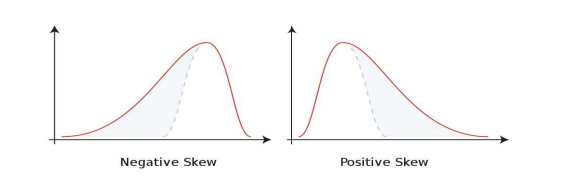
\includegraphics[width=0.6\linewidth]{Figs/C5_1.png}}
	\subfloat[Kurtosis of Distributions]{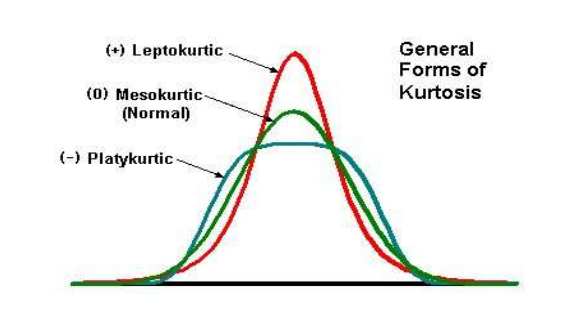
\includegraphics[width=0.4\linewidth]{Figs/C5_2.png}}
    \caption{偏度与峰态}
    \label{fig 5.7.1}
  \end{figure}


\subsection{样本偏度与样本峰度}
根据式 \ref{eq 5.7.1} 和式 \ref{eq 5.7.2} ,用样本三阶矩和四阶矩来计算样本偏度与峰度。样本三阶矩(与样本方差的计算公式相对照)为:
\begin{equation}
     \frac{\sum( \boldsymbol{X-\bar{X}})^{3}}{n-1} 
\end{equation}

样本四阶矩为:
\begin{equation}
    \frac{\sum(\boldsymbol{ X-\bar{X}})^{4}}{n-1}
\end{equation}

前述内容可用于设计正态性的检验。正态分布是对称和常峰态的。对称意味着三阶矩$ \operatorname{E}\boldsymbol{ \varepsilon }^{ 3 } ]$为 0 。分布对称性的标准量是偏态(Skewness)
$$  \sqrt{\beta_{1}}=\frac{\mathbb{E}\left[ \boldsymbol{ \varepsilon }^{3}\right]}{\left(\sigma^{2}\right)^{3 / 2}} $$

峰态(Kurtosis)是分布尾部厚度的度量。此度量是:
$$ \beta_{2}=\frac{\mathbb{E}\left[\boldsymbol{ \varepsilon }^{4}\right]}{\left(\sigma^{2}\right)^{2}} $$

正态分布对于这个度量通常是评价标准;常峰态值是正态分布的峰度,等于 3 。因此,我们可以通过比较偏度是否为 0 和峰度是否为 3 来判断该分布是否为正态分布。在实际中,通常的度量是过量程度(degree of excess)
($ \beta_{2} -3 $) 。我们将使用的工具是一个沃尔德统计量。在正态性的假设下,此检验统计量是:
$$ W=n\left[\frac{b_{1}}{6}+\frac{\left(b_{2}-3\right)^{2}}{24}\right] \sim \chi^{2}(2) $$

称为正态性的哈尔克-贝拉(Jarque-Bera) BJ 检验。

这渐近地服从自由度为 2 的 $ \chi^{2} $分布。这些参数的可行的估计量是利用最小二乘残差计算而得到的。统计量可以参考标准 $ \chi^{2}$表。

由贝拉和哈尔克(1980 a , 1980b )推导的这个检验统计量的皮尔逊分布的内容中是作为拉格朗日乘数检验。应该注意这个检验本质上是无建设性的。非正态性的发现不一定给出
下一步如何做的建议。同样,注意不能拒绝正态性并没有确认了正态性。这只是一个对称性和常峰态的检验。

\section{思考题}

1. 对于线性统计模型 $ \boldsymbol{ y=X \beta+\varepsilon } $。 
假设 $ \varepsilon \sim N\left(0, \sigma^{2} I_{n}\right), n=13, K=3 $,最小化误差平方和 $ \boldsymbol{ (y-X \beta)^{\prime}(y-X \beta)} $
得到如下线性方程组:
$$ \left\{\begin{array}{l}
    b_{1}+2 b_{2}+b_{3} = 3 \\
    2 b_{1}+5 b_{2}+b_{3} = 9 \\
    b_{1}+b_{2}+6 b_{3} = -8
    \end{array}\right. $$
\begin{enumerate}[(1)]
    \item 把这个方程组写成矩阵的形式,并利用矩阵方法求最小二乘估计量$ b $的值。
    \item 如果$ y^{\prime}y = 53 $,求$\sigma^{2} $的无偏估计量 $ s^{2}$ 的值
    \item 求 $ b $ 的协方差矩阵。
    \item 分别写出能够检验 $ H_{0}: \beta_{k}=\beta_{k}^{0} $的 $ t $ 统计量(k=1, 2, 3)。
    \item 写出能够检验$ H_{0}: \beta_{1}+\beta_{2}-2 \beta_{3}=q $ 的 t 统计量和 F 统计量。
\end{enumerate}

2. 假设$ \boldsymbol{ b } $是$ \boldsymbol{ y } $关于$ \boldsymbol{ X } $的回归的最小二乘估计量,$ c $ 是另一$ K \times 1 $向量,证明两个残差平方和之差是:
$$ \boldsymbol{ (y-X c)^{\prime}(y-X c)-(y-X b)^{\prime}(y-X b)=(c-b)^{\prime} X X(c-b)} $$ 

并证明这个差值是正的。

3. 假设对于同一个参数$ \theta $ ,你有两个相互独立的无偏估计量$ \theta^{1} $和$ \theta^{2} $,它们的方差分别为 $ v_{1} $ 和 $ v_{2} $ 且  $ v_{1} \neq v_{1} $  ,
那么什么样的线性组合 $ \hat{\theta}=c_{1} \hat{\theta}_{1}+c_{2} \hat{\theta}_{2} $ 是$ \theta $的最小方差无偏估计量?

4. 假设对于同一个参数$ \theta $ ,你有$ n $个相互独立的无偏估计量 $ \hat{\theta}_{1} \cdots \cdots \hat{\theta}_{n} $,
它们的方差分别 $ v_{1}, \cdots, v_{n} $。那么什么样的线性组合 $ \hat{\theta}=c_{1} \hat{\theta}_{1}+\cdots+c_{n} \hat{\theta}_{n} $是 $ \theta $  的最小方差无偏估计量?